\documentclass[10pt, a4paper]{article}

\usepackage{fancyhdr} 
\usepackage{graphicx}
\usepackage{subcaption}
\usepackage[margin=1.5in]{geometry} 

\title{{\Large Approaches to Human Action Recognition and \\ Three-dimensional Pose Estimation } \\ {\normalsize Progress Report for The Croucher Foundation}}
\author{Tsz-Ho Yu}
\date{\today} 

\begin{document}

\maketitle 

\section{Introduction} 
 
This thesis proposes new techniques for the automatic analysis of human activities in videos. We address the three high-level sub-problems of human activity analysis: \emph{action recognition}, \emph{3-D body pose estimation} and \emph{3-D hand pose recognition}. 

Our primary contributions are threefold. Firstly, we propose a novel method to classify human actions in real-time using spatioetmporal semantic and structural forests. Secondly, we address the problem of 3-D human body pose estimation by combining a deformable part model and a novel action detection forest. Thirdly, detailed 3-D hand poses are estimated from depth maps using a regression random forest and an efficient data-driven kinematic pose refinement framework.      

\section{Evaluation of Volumetric Feature Detectors}

Feature detection is the first and most crucial step of many computer vision tasks, including object recognition, object reconstruction and tracking. This thesis aims to conduct a performance evaluation of interest point detectors on scalar volumetric data for action recognition and human pose estimation tasks. 

%or inside dense voxels with varying intensities. 
%Furthermore, the nature of the data---voxels, the 3D equivalent of pixels---makes repurposing the many 2D interest point detectors for 3D straightforward. 

\begin{figure}[h]
\centering
\subcaptionbox{DoG}{
	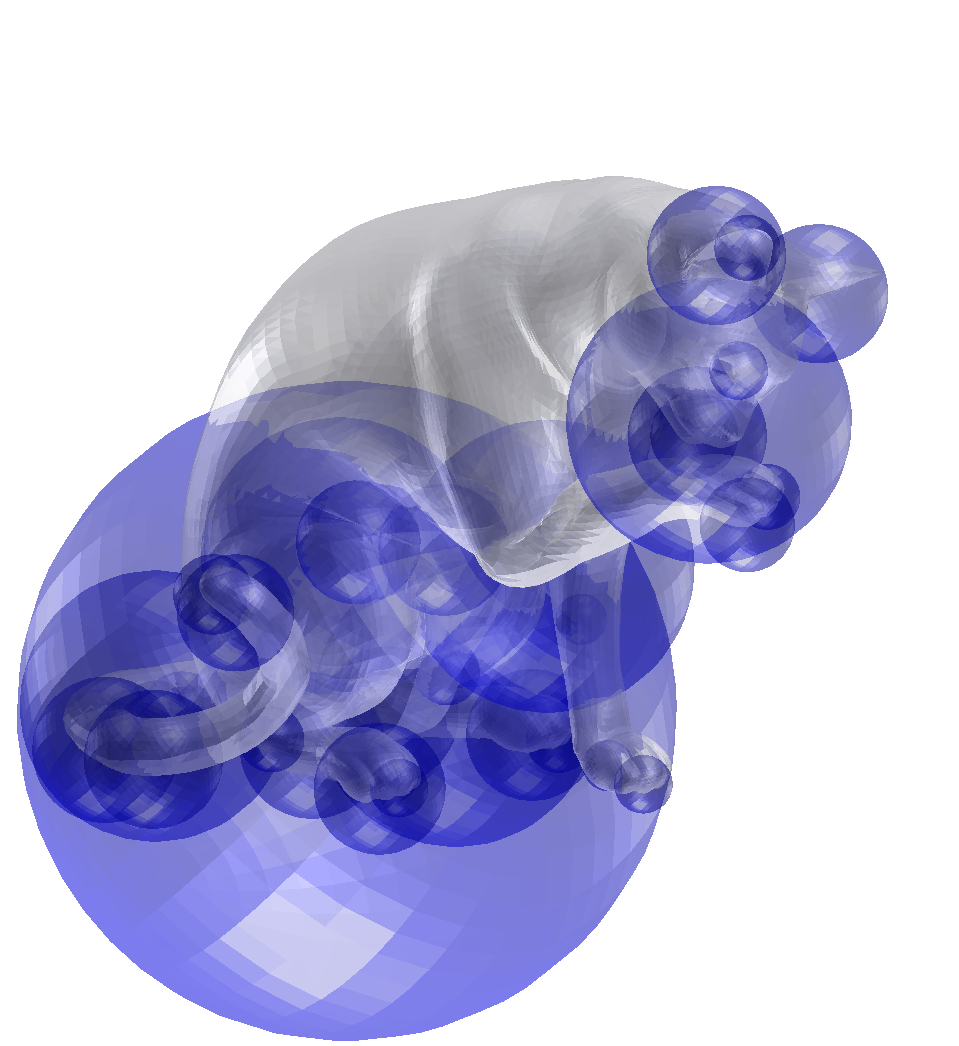
\includegraphics[width=0.16\linewidth]{fig/eval/cat_dog.png} \hspace{-3mm}
	\label{fig:testshapes:dog}
}
\hspace{-3.5mm}
\subcaptionbox{SURF}{
	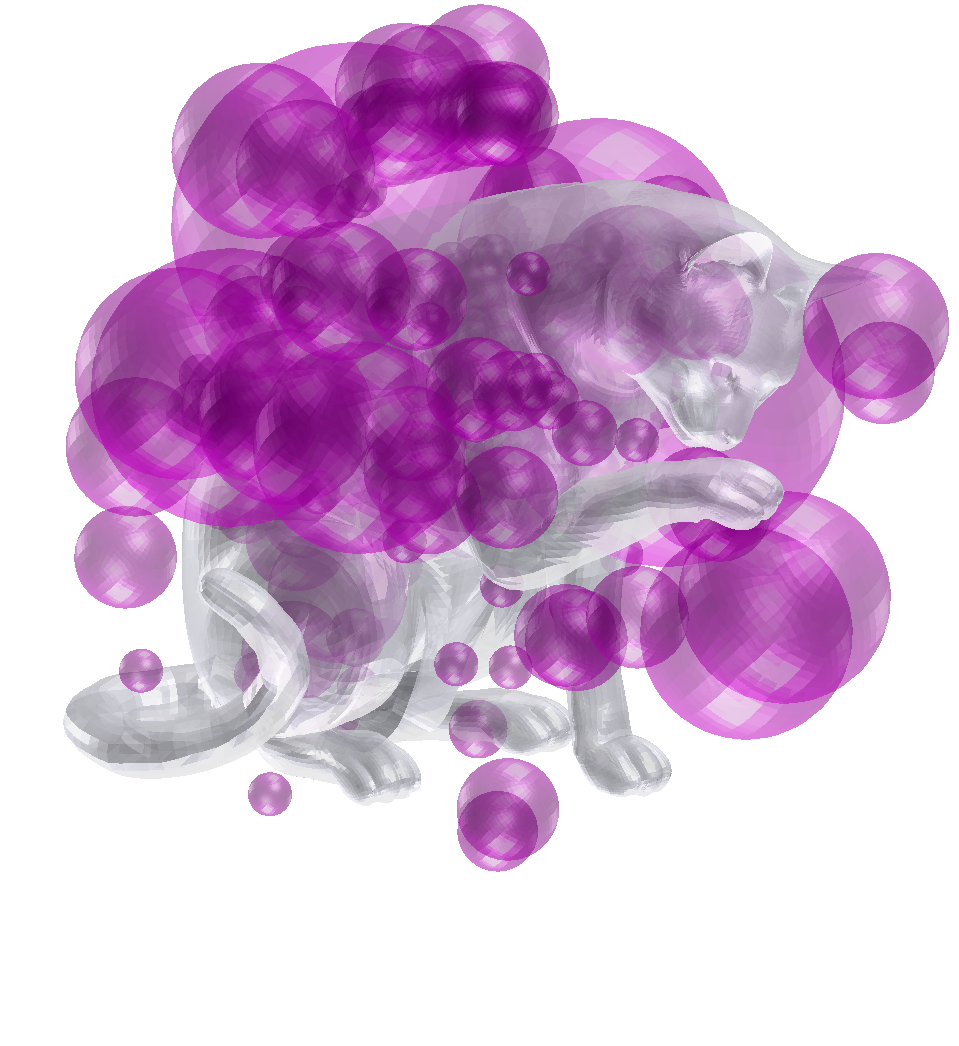
\includegraphics[width=0.16\linewidth]{fig/eval/cat_surf.png} \hspace{-3mm} 
	\label{fig:testshapes:surf}
}
\hspace{-3.5mm}
\subcaptionbox{Harris}{
	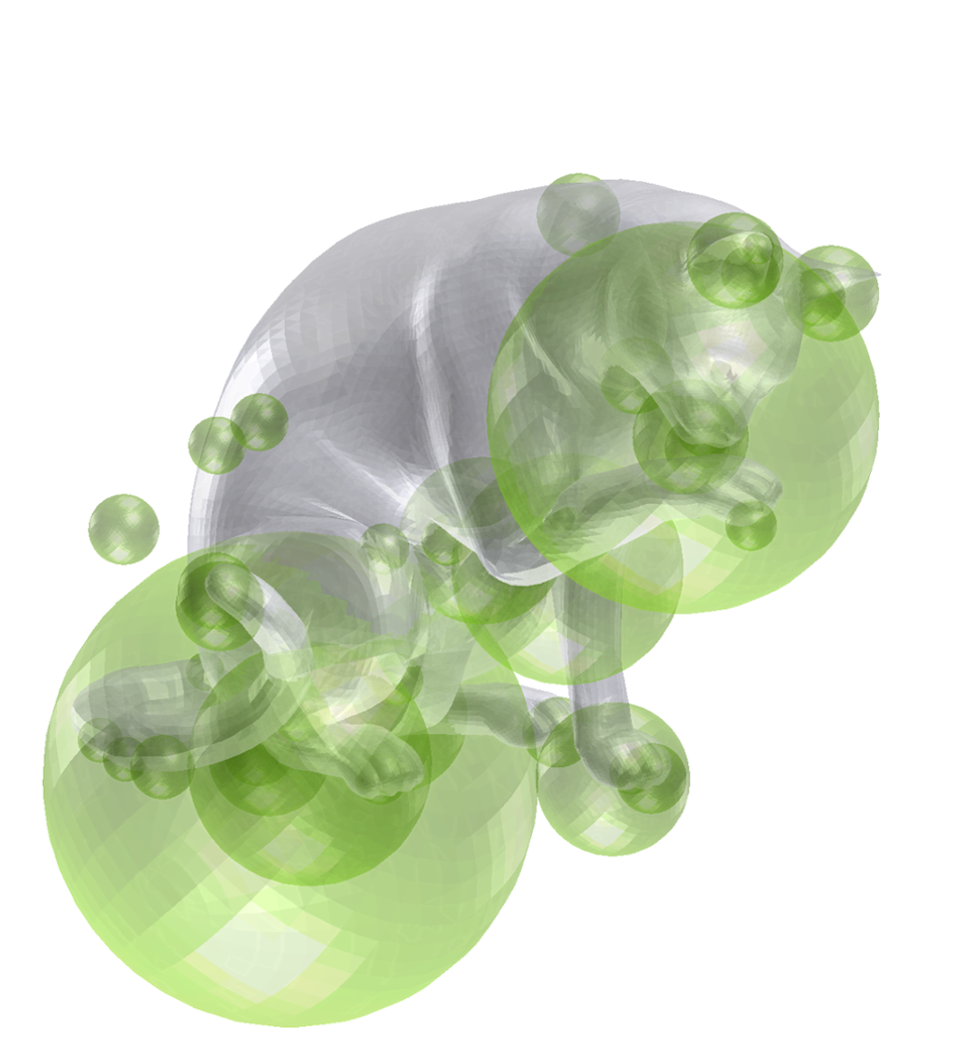
\includegraphics[width=0.16\linewidth]{fig/eval/cat_harris.png} \hspace{-3mm}
	\label{fig:testshapes:harris}
}
\hspace{-3.5mm}
\subcaptionbox{DoH}{
	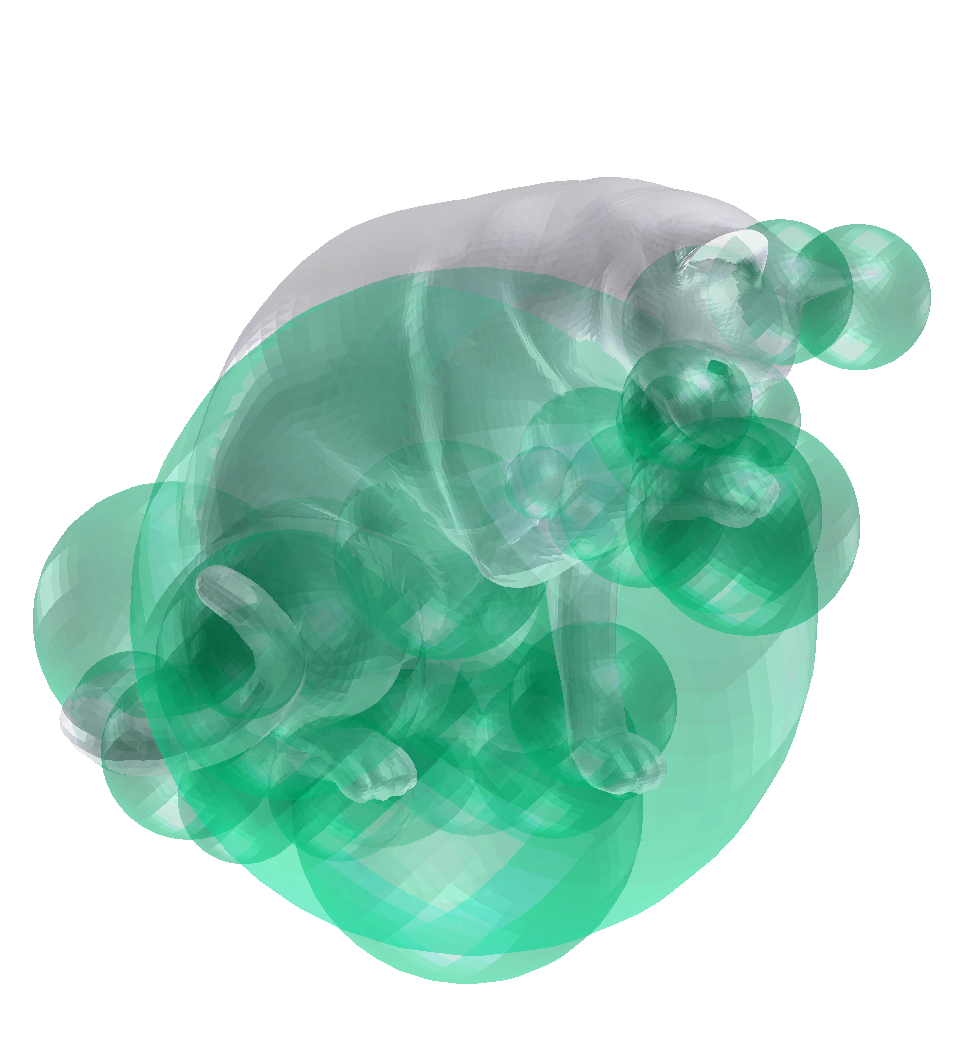
\includegraphics[width=0.16\linewidth]{fig/eval/cat_hessian.png} \hspace{-3mm}
	\label{fig:testshapes:hessian}
}
\hspace{-3.5mm}
\subcaptionbox{V-FAST}{
	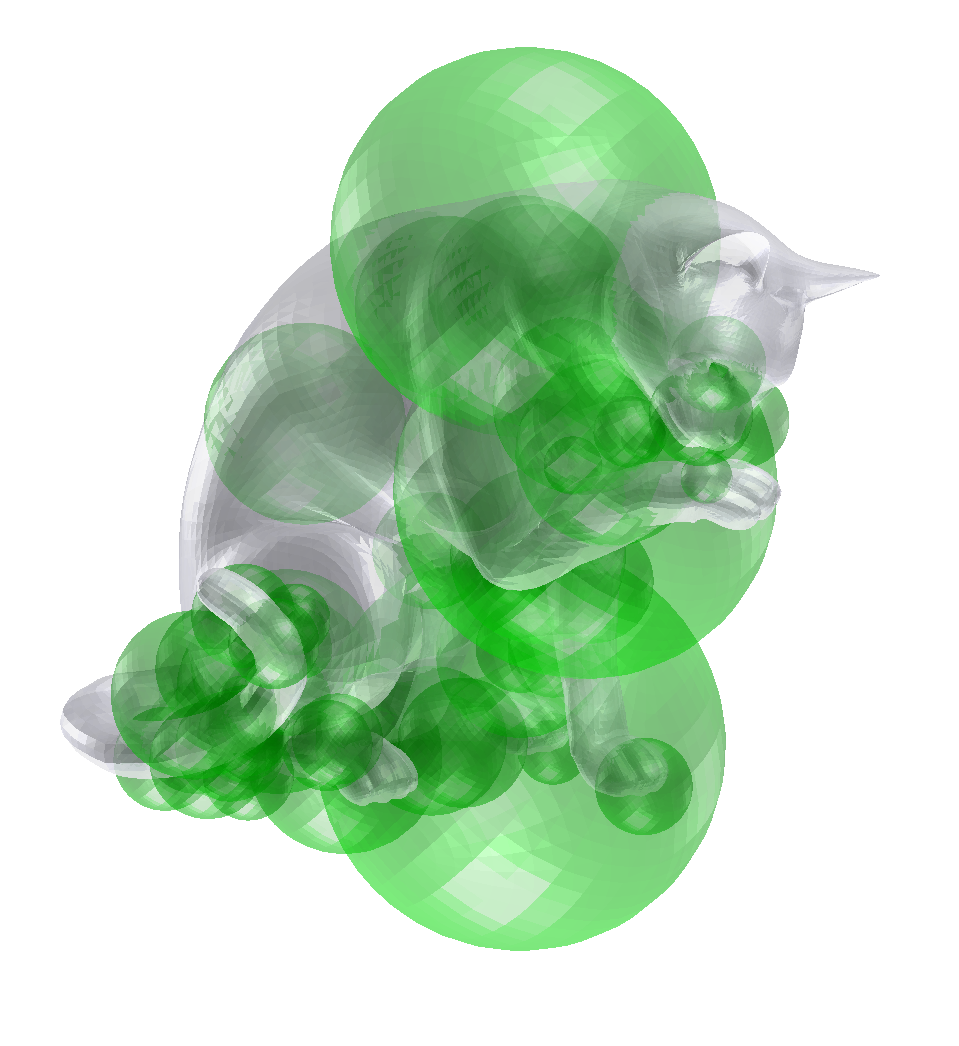
\includegraphics[width=0.16\linewidth]{fig/eval/cat_fast.png} \hspace{-3mm}
	\label{fig:testshapes:fast}
}
\hspace{-3.5mm}
\subcaptionbox{MSER}{
	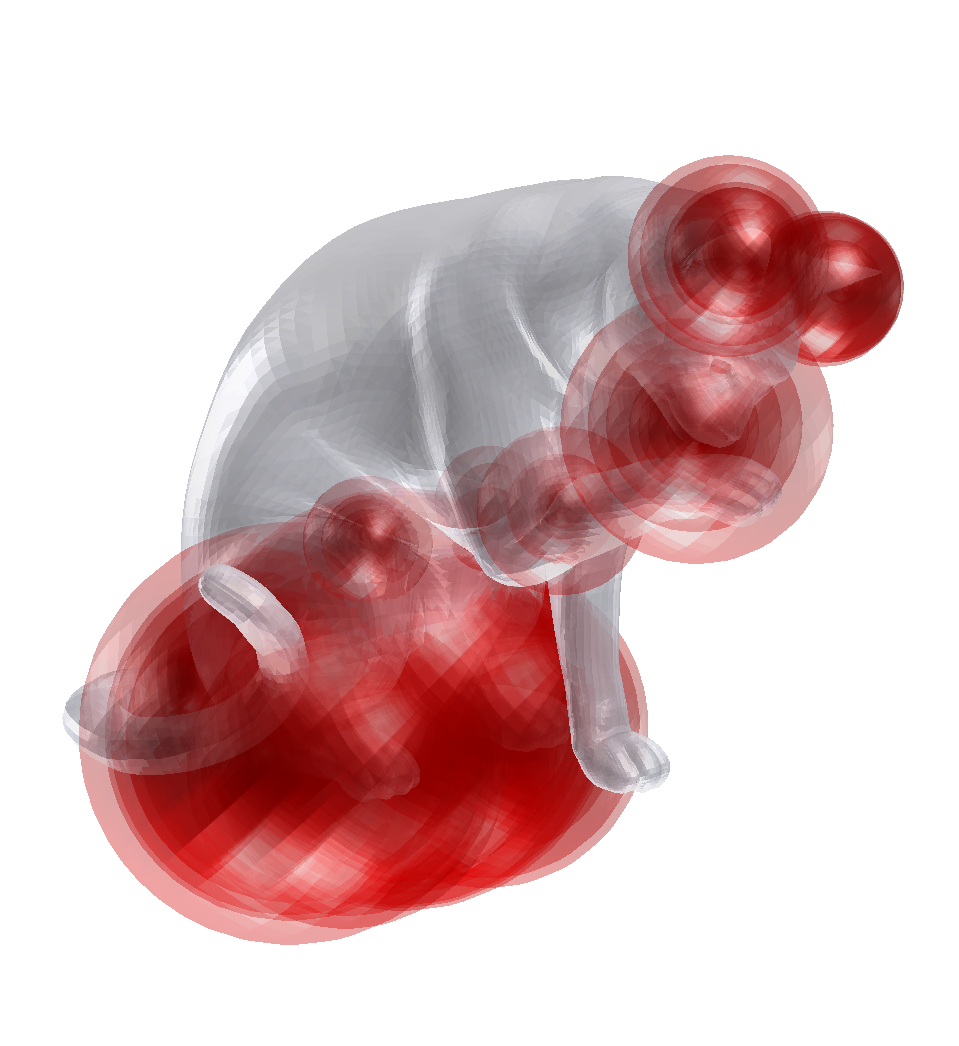
\includegraphics[width=0.16\linewidth]{fig/eval/cat_mser.png}
	\label{fig:testshapes:mser}
}
\caption{\label{fig:testshapes}Different types of volumetric interest points detected on a test shape.}
\end{figure}

The state of the art in volumetric interest point detection is evaluated. The purpose of this work is to provide comprehensive guidance on the selection of interest point detector for any computer vision or machine learning task that uses 3D input data. Six interest point detectors (see figure \ref{fig:testshapes}), from existing 3D computer vision applications, are evaluated on three different datasets (meshes, MRI scans and 3D point clouds) under varying noise levels and transformations. 

A novel evaluation metric is introduced by combining two existing performance metrics, repeatability and accuracy, into a single measurement. The acquired experimental results are analyzed both quantitatively and qualitatively. This project has been published in the Proceedings of 3DIMPVT \cite{Yu2011} and International Journal of Computer Vision \cite{Yu2013b}. 

\section{Action Recognition}

A novel solution for action classification is presented in our work. Different from other published approaches, a major strength of our method is the run-time speed. Real-time performance is achieved by \emph{semantic texton forest (STF)} which works on video pixels generating visual codewords in an extremely fast manner. 

The new MpSRM algorithm is proposed to capture both spatiotemporal structures and local-appearances of actions and ease quantisation effects based on STF. Furthermore, a novel fast interest point detector and application of random forest and kernel k-means forest classifiers contribute to the acceleration of recognition speed.

\begin{figure}[ht]
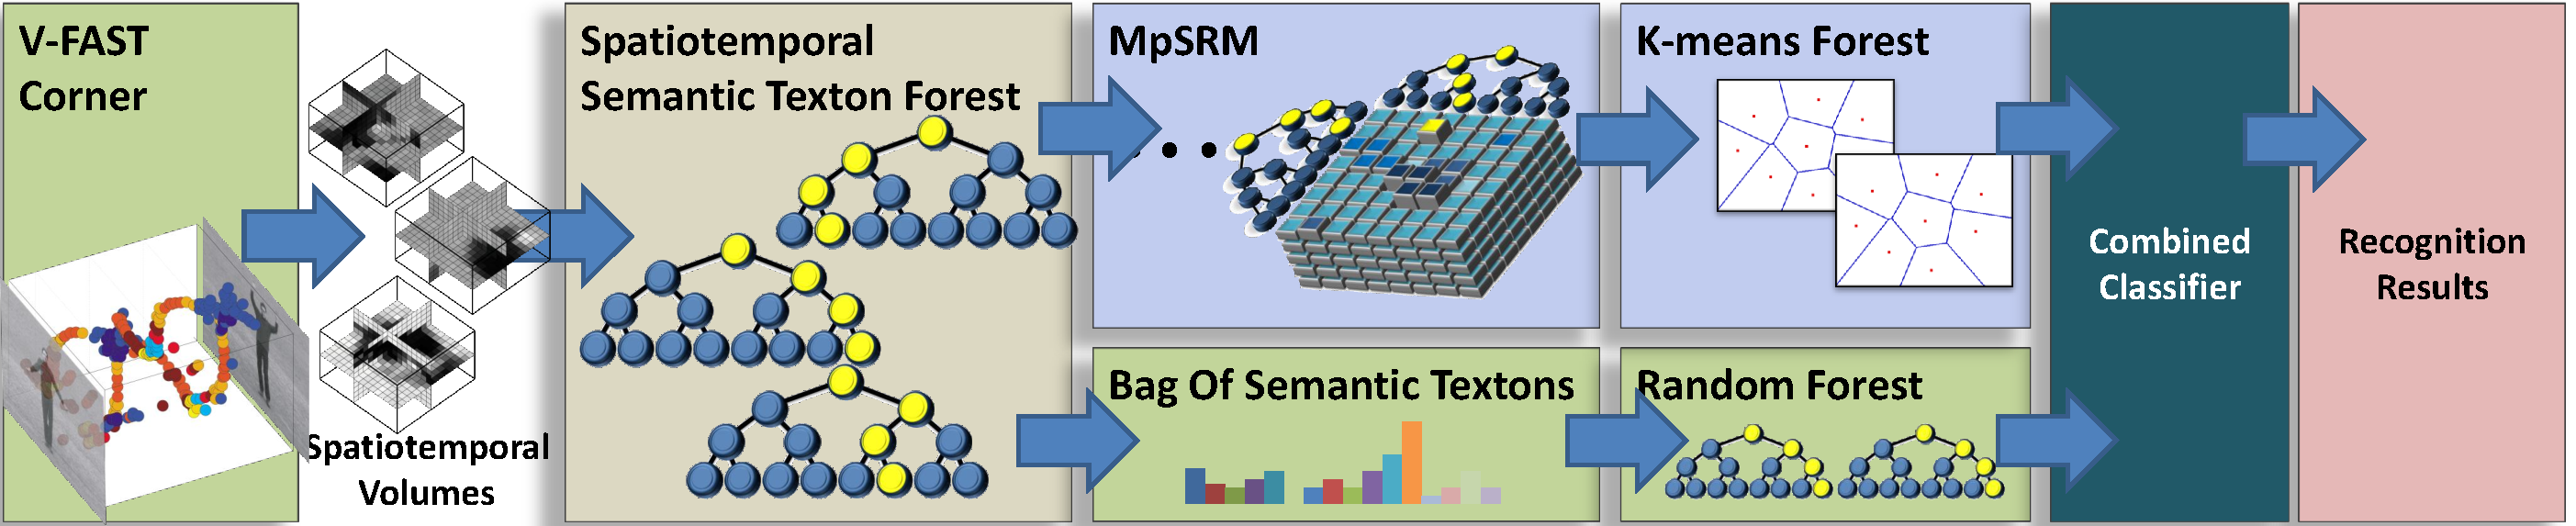
\includegraphics[width=1.0\linewidth]{fig/act/fig1_new.pdf}%flow.png}
\caption{Overview of the proposed approach}
\label{fig/act/flow}
\end{figure}

\begin{figure}[ht]
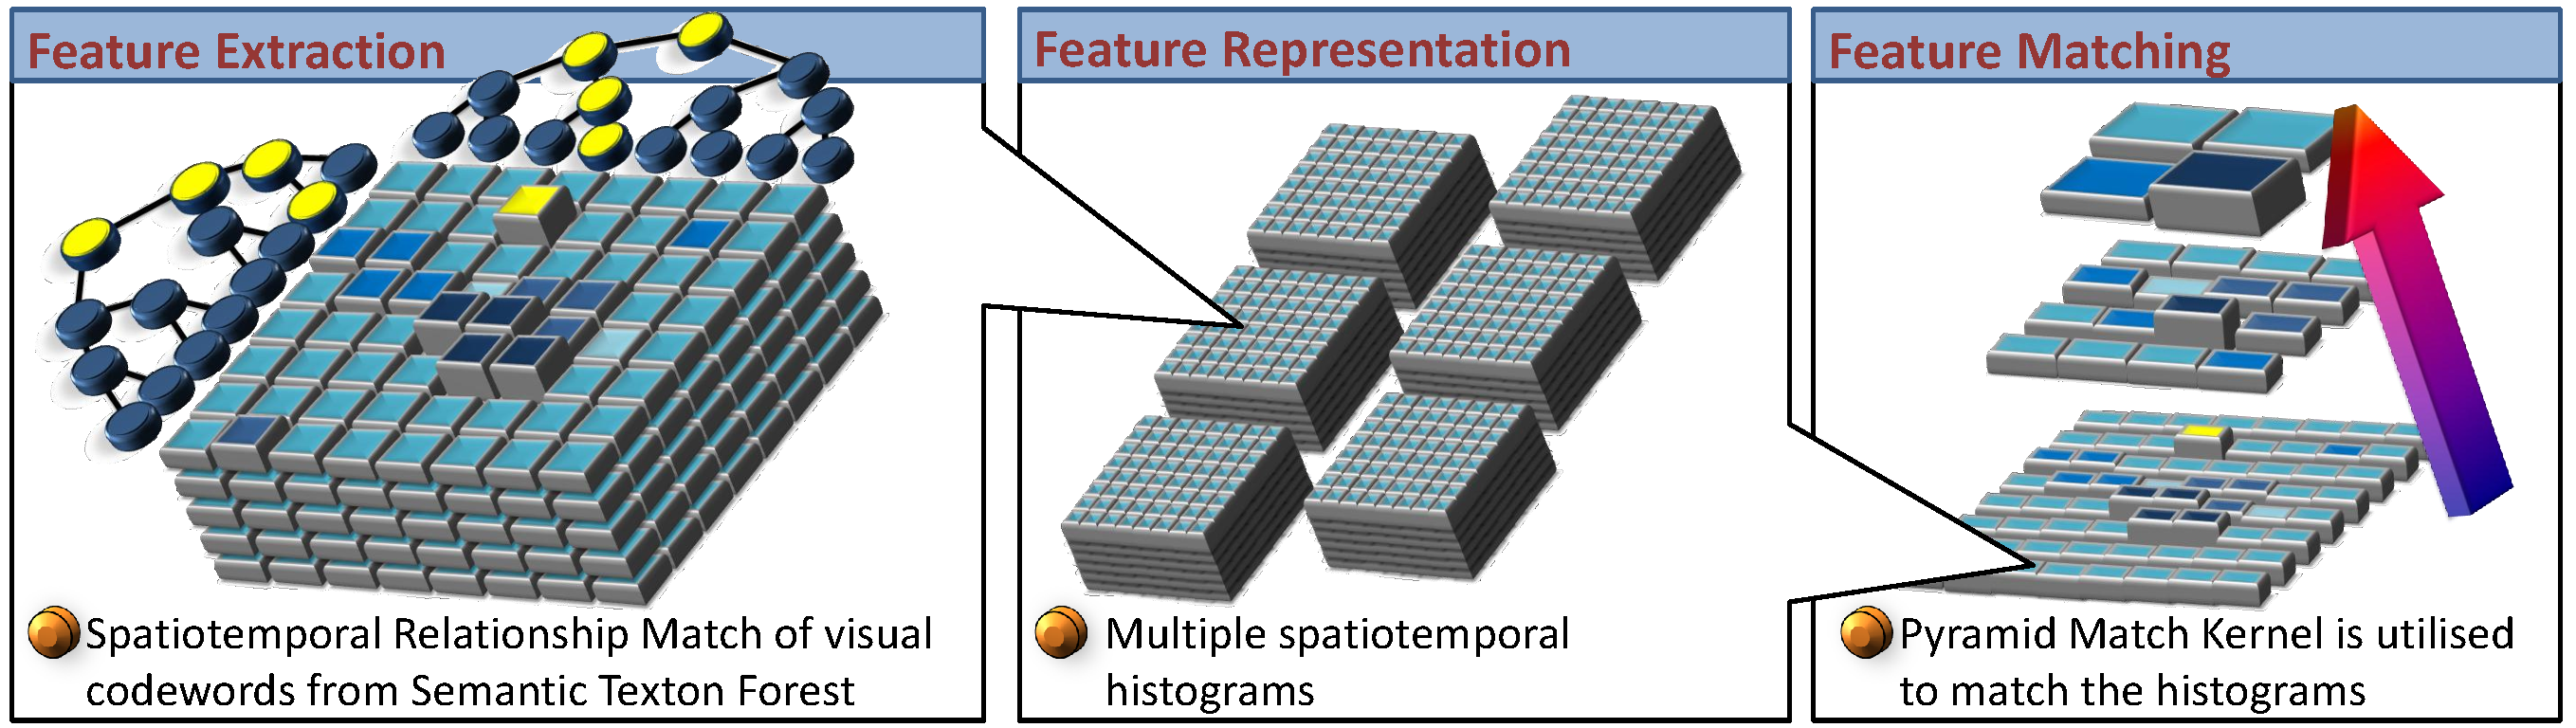
\includegraphics[width=1\linewidth]{fig/act/fig4.pdf}%mpsrm.png}
\caption{Multi-pyramidal spatiotemporal relationship match (MpSRM)}
\label{fig/act/mpsrm}
\end{figure}

Different from other published approaches, a major strength of our method is the run-time speed. Real-time performance is achieved by semantic texton forest which works on video pixels generating visual codewords in an extremely fast manner. MpSRM is proposed to capture both spatiotemporal structures and local-appearances of actions and ease quantisation effects based on STF. Furthermore, a novel fast interest point detector and application of random forest and kernel k-means forest classifiers contribute to the acceleration of recognition speed. 

Experimental results show the comparable accuracies of the proposed method compared to state-of-the-arts. A future challenge will be tackling more complex realistic human actions and partial occlusions, as well as requiring continuous action localisation with a real-time performance. This project has been published in the Proccedings of the British Machine Vision Conference 2010 (BMVC 2010) \cite{Yu2010}.  

\section{3-D Body Pose Estimation}

This work addresses the challenging problem of unconstrained 3D human pose estimation (HPE) from a novel perspective. Existing approaches struggle to operate in realistic applications, mainly due to their scene-dependent priors, such as background segmentation and multi-camera network, which restrict their use in unconstrained environments.

\begin{figure}[ht]
	\centering
	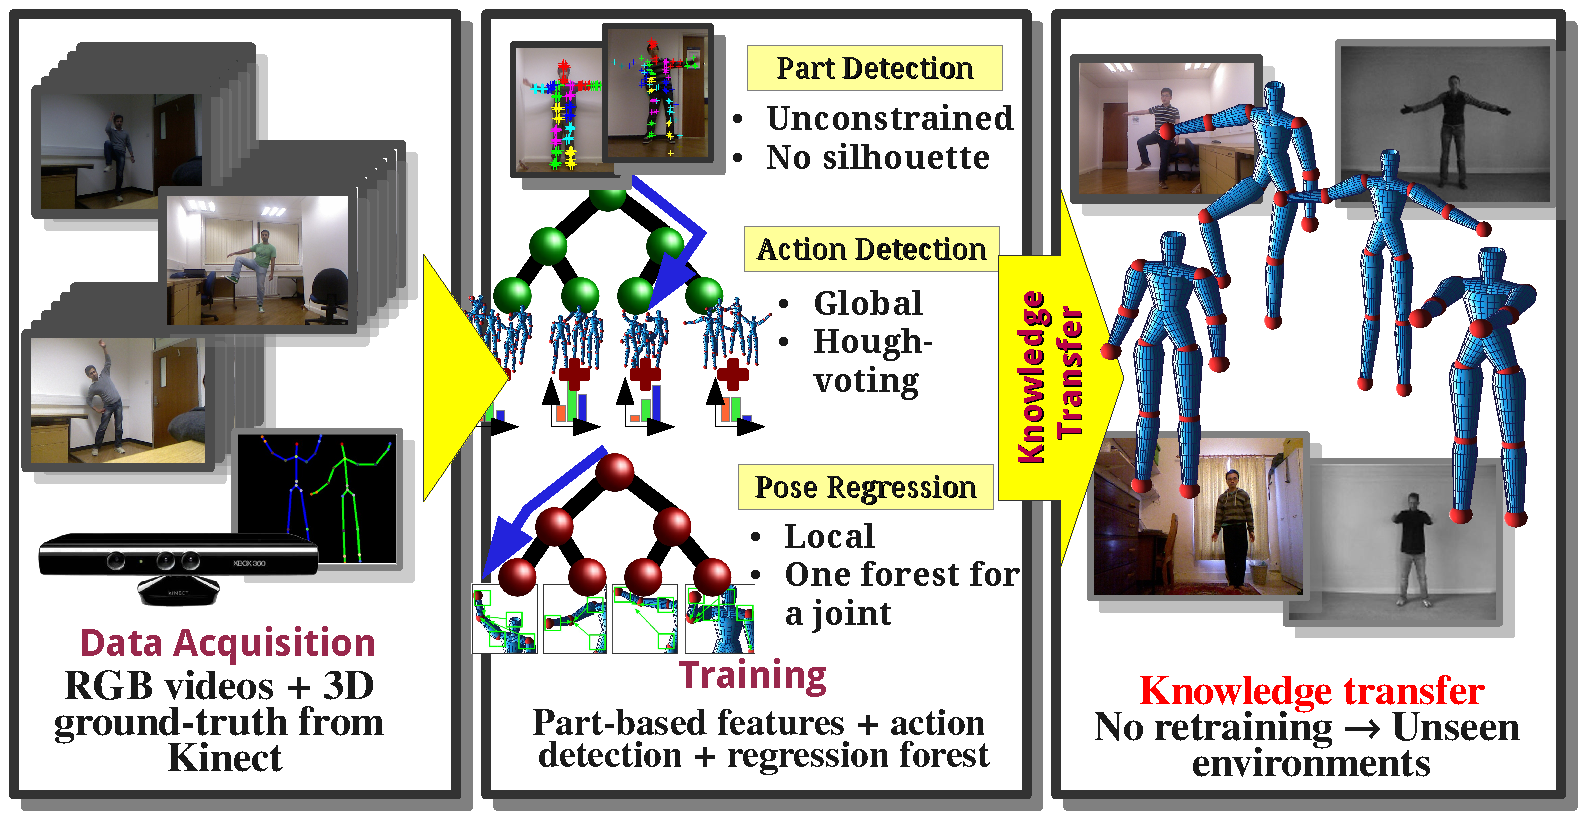
\includegraphics[width=1\linewidth]{fig/body/figure2_transferexplain.pdf}
	\caption{Overview of the proposed 3-D pose estimation framework} 
	\label{fig/body/transferexplain}
\end{figure}

We therfore present a framework which applies action detection and 2D pose estimation techniques to infer 3D poses in an unconstrained video. Action detection offers spatiotemporal priors to 3D human pose estimation by both recognising and localising actions in space-time. Instead of holistic features, e.g. silhouettes, we leverage the flexibility of deformable part model to detect 2D body parts as a feature to estimate 3D poses. A new unconstrained pose dataset has been collected to justify the feasibility of our method, which demonstrated promising results, significantly outperforming the relevant state-of-the-arts. The above 3-D body pose estimation project will be published in the coming Proceedings of the 2013 Conference of Computer Vision and Pattern Recognition (CVPR) \cite{Yu2013}. 

\section{3-D Hand Pose Estimation} 

\begin{figure}[!ht] 
	\centering
	\begin{tabular}{cccc}
		Input & Depth Map & Labels & Ours \\ 
		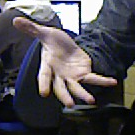
\includegraphics[width=2.7cm]{fig/hand/qual/rgb/image_0303.png} &
		
\includegraphics[width=2.7cm]{fig/hand/qual/depth/image_0303.png} &
		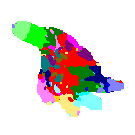
\includegraphics[width=2.7cm]{fig/hand/qual/class/class-303.png} &
		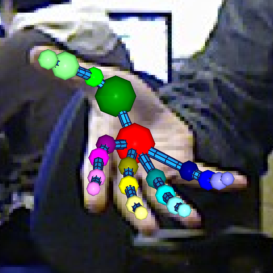
\includegraphics[width=2.7cm]{fig/hand/qual/vote/image_0303.png}
		\phantomsubcaption\label{fig/hand/multi1} \\ 
		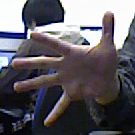
\includegraphics[width=2.7cm]{fig/hand/qual/rgb/image_0520.png} &
		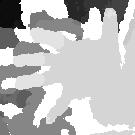
\includegraphics[width=2.7cm]{fig/hand/qual/depth/image_0520.png} &
		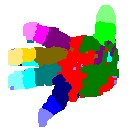
\includegraphics[width=2.7cm]{fig/hand/qual/class/class-520.png} &
		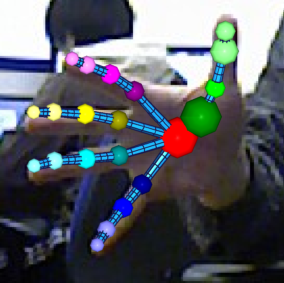
\includegraphics[width=2.7cm]{fig/hand/qual/vote/image_0520.png}
		\phantomsubcaption\label{fig/hand/multi2} \\
		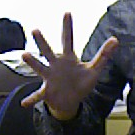
\includegraphics[width=2.7cm]{fig/hand/qual/rgb/image_0996.png} &
		
\includegraphics[width=2.7cm]{fig/hand/qual/depth/image_0996.png} &
		
\includegraphics[width=2.7cm]{fig/hand/qual/class/class-996.png} &
		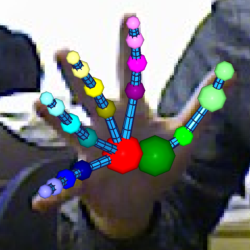
\includegraphics[width=2.7cm]{fig/hand/qual/vote/image_0996.png}
		\phantomsubcaption\label{fig/hand/multi5} \\ 
	\end{tabular}
	\caption{3-D hand pose estimation results of the proposed algorithm. }
\end{figure} 

This project presents the first semi-supervised transductive approach for articulated hand pose estimation.  
Despite its similarity with body pose estimation, techniques for articulated hand pose is still far from mature, primarily due to the unique issues of occlusion and noise issues in hand pose data. 
On the other hand, the discrepancies between realistic and synthetic data also undermine the performances of state-of-the-arts. 


Addressing the aforementioned issues, we propose a novel discriminative approach, \emph{Semi-supervised Transductive and Regression (STR)} forest, to estimate hand articulations using both realistic and synthetic data. With transductive learning, the STR forest recognises a wide range of poses from a small number of labelled realistic data. Semi-supervised learning is applied to fully utilise the sparsely labelled realistic dataset. Besides, we also present a data-driven pseudo-kinematic technique, as means to improve the estimation accuracy of occluded and noisy hand poses. 

The proposed approach is evaluated with respect to different challenging environments.    
From the quantitative and qualitative analyses conducted, our method has demonstrated promising results in estimating articulated hand poses from noisy and strongly occluded data.  
It also attains superior performances and speed compared with state-of-the-art. This project has been submitted for publlication \cite{Tang2013}.  

\bibliographystyle{unsrt}
\bibliography{references} 

\end{document} 
